\documentclass[a4paper,12pt]{article}
\usepackage[utf8]{inputenc}
\usepackage[spanish,es-tabla]{babel}
\usepackage{color}
\usepackage{parskip}
\usepackage{graphicx}
\usepackage{multirow}
\usepackage{listings}
\usepackage{vmargin}
\graphicspath{ {imagenes/} }
\definecolor{mygreen}{rgb}{0,0.6,0}
\definecolor{lbcolor}{rgb}{0.9,0.9,0.9}
\usepackage{epstopdf}

\lstset{
%backgroundcolor=\color{lbcolor},
    tabsize=4,    
%   rulecolor=,
    language=[GNU]C++,
        basicstyle=\tiny,
        aboveskip={1.5\baselineskip},
        columns=fixed,
        showstringspaces=false,
        extendedchars=false,
        breaklines=true,
        prebreak = \raisebox{0ex}[0ex][0ex]{\ensuremath{\hookleftarrow}},
        frame=single,
        showtabs=false,
        showspaces=false,
        showstringspaces=false,
        identifierstyle=\ttfamily,
        keywordstyle=\color[rgb]{0,0,1},
        commentstyle=\color[rgb]{0.026,0.112,0.095},
        stringstyle=\color{red},
        numberstyle=\color[rgb]{0.205, 0.142, 0.73},
        numbers = left
 %       \lstdefinestyle{C++}{language=C++,style=numbers}’.
}

\begin{document}
\title{Ataque de Buffer Overflow}
\author{
Christofer Fabián Chávez Carazas \\
\small{Universidad Nacional de San Agustín} \\
\small{Seguridad Computacional}
}

\maketitle

\section{Descripción del Experimento}

El experimento consiste en provocar un \textit{buffer overflow} paso a paso, ver el manejo de la memoria y los
problemas que genera, y cómo podemos utilizar el ataque a nuestro favor. El programa que se utilizó para el
experimento se muestra a continuación. Para ver el paso a paso se utilizó el programa \textit{gdb}. Todo el experimento
se realizó en una máquina virtual con ubuntu 32-bits con 1 Gb de memoria RAM.

\begin{lstlisting}
#include <stdio.h>

int read_req(void){
	char buf[128];
	int i;
	gets(buf);
	i = atoi(buf);
	return i;
}

int main(int ac, char ** av){
	int x = read_req();
	printf("x=%d\n",x);
}
\end{lstlisting}

\section{Programa}

El programa a ejecutar consiste en una simple función. Comienza creando un buffer de 128 bytes de tamaño. Luego
se le pide al usuario que ingrese un dato y se almacena en el buffer. Después se convierte el buffer en un entero para
luego retornarlo e imprimirlo en pantalla. En la Tabla \ref{table:res} se muestra una lista de entradas que se 
le dio al programa y lo que imprimió el programa para cada una. Cuando nosotros ponemos un número muy grande
bota un resultado muy diferente, esto se debe a que el número es truncado para que pueda entrar dentro de la variable
\textit{i}. La función \textit{atoi()} itera la cadena de caracteres buscando un dígito, si encuentra algo que no
lo es deja de iterar. Por esta razón cuando ingresamos ``12345AAA'', la función itera hasta encontrar la primera 'A'
y devuelve 12345 como respuesta. En el caso de la entrada ``AAAAAAAAA'', la función termina en la primera iteración
retornando 0 como respuesta. La última entrada de la tabla hace que el programa termine por un desbordamiento de buffer,
esto ocurre porque la entrada es más grande que el buffer, en el caso del experimento, una cadena de 130 ases.

\begin{table}
\begin{center}
 \begin{tabular}{|c|c|}
  \hline
  Input & Output \\
  \hline \hline
  12345 & 12345 \\ \hline
  123456789123456789 & 2147483647 \\ \hline
  12345AAA & 12345 \\ \hline
  AAAAAAAAAAA &  0 \\ \hline
  130 veces 'A' & Error (stack smashing detected) \\ \hline
 \end{tabular}
\end{center}
\caption{Resultados que arroja el programa}
\label{table:res}
\end{table}

\section{Paso a Paso}

Abrimos el programa con \textit{gdb} y colocamos un \textit{breakpoint} al inicio de la función \textit{read\_req()}.
Corremos el programa hasta antes de que se ejecute la función \textit{gets()}. En la Figura \ref{fig:1} se muestran
los registros, generados por el comando \textit{info registers}, y podemos ver la dirección de nuestra pila 0xbfffeee0.
En la Figura \ref{fig:2} podemos ver la dirección de memoria del inicio del buffer 0xbfffeeec y la dirección de la variable
\textit{i} 0xbfffeee8. Analizando estas direcciones, nuestra pila comienza con la dirección de retorno en bfffeee0 hasta
bfffeee8 donde comienza la variable \textit{i}. Esta variable termina en bfffeeec donde comienza el buffer.
Continuamos con la ejecución del programa y ponemos 181 veces la letra 'A'. En la figura \ref{fig:3} se puede ver
que la dirección del buffer está lleno de letras 'A'. Lo que pasa en esta situación es que se desborda el buffer de nuestro
programa y llena la dirección de retorno, y al intentar leer esta dirección ocurre un error. \par

Al volver a correr el programa hasta antes de que el programa bote el error, cambiamos la dirección de retorno a la del main.
Lo que pasa en este caso es que si imprime el valor sólo que ya no tiene otro valor de retorno y vuelve a botar error.
Este ataque es muy explotable ya que, al desbordar el buffer, se puede poner un nuevo puntero en la dirección de retorno que
direccione el programa a una función maliciosa.

\section{Conclusiones}

\begin{itemize}
 \item El buffer overflow es uno de los ataques más explotables y manipulables.
 \item Siempre hay que verificar el tamaño que se guarda en un buffer.
\end{itemize}


\begin{figure}[b]
 \centering
 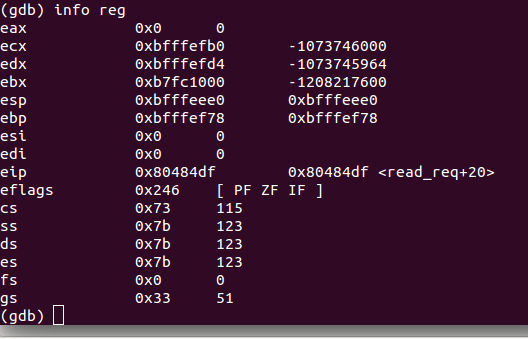
\includegraphics[scale=0.5]{1.png}
 \caption{Registros antes del \textit{gets()}}
 \label{fig:1}
\end{figure}

\begin{figure}
 \centering
 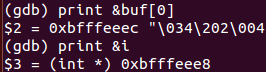
\includegraphics[scale=1]{2.png}
 \caption{Direcciones del inicio del buffer y la variable \textit{i}}
 \label{fig:2}
\end{figure}

\begin{figure}
 \centering
 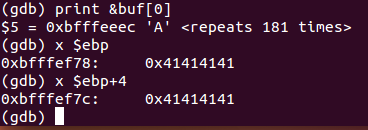
\includegraphics[scale=0.7]{3.png}
 \caption{Registros de la pila}
 \label{fig:3}
\end{figure}

\end{document}
